\chapter[Software for fitting evolutionary models to phylogenetic data]{Software for fitting evolutionary models to phylogenetic data\footnote{Previously published as: Pennell, M.W., J.M. Eastman, G.J. Slater, J.W. Brown, J.C. Uyeda,
  R.G. FitzJohn, M.E. Alfaro, and L.J. Harmon. 2014.
  geiger v2.0: an expanded suite of methods for fitting macroevolutionary
  models to phylogenetic trees. Bioinformatics 15:2216--2218.}} 
\label{chap:geiger}

\section{Summary}
Phylogenetic comparative methods are essential for addressing evolutionary hypotheses with interspecific data. The scale and scope of such data has increased dramatically in the last few years. Many existing approaches are either computationally infeasible or inappropriate for data of this size. To address both of these problems, we present \textsc{geiger v2.0}, a complete overhaul of the popular R package \textsc{geiger} \citep{Harmon2008}. We have re-implemented existing methods with more efficient algorithms and have developed several new approaches for accomodating heterogeneous models and data types.  


\section{Introduction}

In the past few decades, phylogenetic trees have become an key component of evolutionary research. This development has been fueled by the increased availability of robust time-calibrated phylogenies for many groups, in addition to an expanding number of statistical techniques for inferring patterns and processes from comparative data \citep[reviewed in][]{PennellHarmon}. Among the many R packages developed for phylogenetic and comparative data, \textsc{geiger} \citep{Harmon2008} has been a primary utility for making macroevolutionary inferences from phylogenetic trees. 

However, in the 6 years since the initial release of \textsc{geiger}, the data available for comparative biology have changed substantially. For some groups, we now have phylogenies and corresponding trait data with thousands (and even tens of thousands) of species \citep[e.g.,][]{Jetz2012, Rabosky2012, PyronBurbrink2013, ksi,Zanne}. \textsc{geiger v2.0} is a complete overhaul of the previous release \citep{Harmon2008}, designed to scale up comparative methods to large data sets. To do so,  we have taken two complementary tacks. The first is to improve algorithms and implementations to increase computational efficiency of existing methods. The second is to expand the suite of statistical approaches to allow for heterogeneity in both models and data types across the phylogeny.  

In this chapter, we briefly describe the methods now in \textsc{geiger}, with a particular focus on novel implementations and algorithms. Most of these methods have been previously published elsewhere in some form and we refer readers to the relevant publications for full explanations. For an overview of the main features of the package, see Table \ref{tab:geiger-fxns}.

\begin{table}
\centering
  \begin{tabular}{| p{3.5cm} | p{5.5cm} | p{4cm} |}
    \hline
    Function & Description & Citations \\ \hline
    \texttt{fitContinuous} & Fit continuous trait models with ML & \citet{Felsenstein1973, Hansen1997, Pagel1997, Pagel1999, Blomberg2003, Hunt2006, Harmon2010, FitzJohn2012} \\ \hline
    \texttt{fitDiscrete} & Fit discrete trait models with ML & \citet{Pagel1994, Lewis2001, FitzJohn2009} \\ \hline
    \texttt{rjmcmc.bm} & Fit multi-rate models to continuous traits & \citet{Eastman2011} \\ \hline
    \texttt{rjmcmc.bm} & Fit jump diffusion models to continuous traits & \citet{Eastmanjump} \\ \hline
    \texttt{mecca} & Fit continuous models to unresolved clades with ABC & \citet{Slater2012MECCA} \\ \hline
     \texttt{fitContinuousMCMC} & Fit simple models of continuous trait evolution with MCMC and incorporate fossil data & \citet{Slater2012Fossil} \\ \hline
     \texttt{pp.mcmc} & Posterior predictive simulations to assess model adequacy & \citet{SlaterPennell} \\ \hline
    \texttt{medusa} & Estimate shifts in diversification rates & \citet{Alfaro2009} \\ \hline
     \texttt{congruify.phylo} & Time-scale large phylogenies & \citet{Eastman2013} \\ \hline
  \end{tabular}
\caption[Major features of geiger v2.0]{Major functions of \textsc{geiger v2.0} with description and citations}
\label{tab:geiger-fxns}
\end{table}



\section{Methods}
\subsection{Fitting simple models of character evolution with maximum likelihood}

Fitting and comparing  models of trait evolution can provide insight into many macroevolutionary questions \citep{PennellHarmon}. The two ``workhorse'' functions in \textsc{geiger} for fitting models of trait evolution using maximum likelihood, \texttt{fitContinuous} and \texttt{fitDiscrete}, have both been completely re-implemented. The previous version of \texttt{fitContinuous} calculated the likelihood of a set of continuous characters (e.g., body size) having evolved under a model using a variance-covariance (vcv) matrix approach. This involves inverting the vcv, which is extremely computationally intensive, making the method infeasible for large trees \citep{Hadfield2010, FitzJohn2012, Freckleton2012, Ho2014}. \citet{FitzJohn2012} demonstrated that using a ``pruning''-based algorithm \citep{Felsenstein1973} allows for much more efficient likelihood calculations. This algorithm is used the \textsc{diversitree} package \citep{FitzJohn2012}. (For related algorithms, see \citealt{Freckleton2012}, \citealt{Ho2014}). The approach has now been extended to all the models in \texttt{fitContinuous}. In addition to improving the efficiency of the algorithm, we have improved numerical optimization procedures and implemented a novel method to simultaneuously estimate model parameters and an additional term to account for measurement error.

For discrete character data (for example, the presence or absence of fur), the most commonly used model is the Mk model \citep{Pagel1994, Lewis2001}.  In this model, there are $n$ states $1, 2, ..., n$ and the goal is to estimate rates of
transition among these, where the rate of transition from state $i$ to
state $j \neq i$ is $q_{ij}$.  Considering just one branch in a
phylogeny, let $\vec D$ be the vector of probabilies of the data given
we are in state $i$, that is, the $i$th element of $D$ is the
probability of the data descended from this point in the tree, given
that we are in state $i$; see \citet{Maddison2007} and \citet{FitzJohn2012}
for notation.

In most R-based implementations of Mk, e.g., \textsc{ape} \citep{ape}
and previous versions of \textsc{geiger} \citep{Harmon2008} to move from the
tip to the base of a branch, we multiply $\vec D$ by $\mathbf{P}(t)$: the
transition probability matrix with off--diagonal elements that describe
the probability of moving from state $i$ to state $j$ over time $t$
and diagonal elements that describe the probability of not changing
from state $i$.  To compute $P(t)$, we take the transition rate matrix
$\mathbf{Q}$ composed of $q$ parameters above and compute
$\mathbf{P}(t) = \exp(\mathbf{Q} t)$ where $\exp$ is the matrix
exponential \citep{Sidje-1998-130}.

For \textsc{geiger v2.0} we have sped up these calculations by using an alternative algorithm.
As the number of states gets very large, it is simpler to compute
$\exp(\mathbf{Q}t) \vec D$ directly, rather than in two steps
\citep{Sidje-1998-130}.  This can be done by solving the system of
differential equations
\begin{equation}
\frac{d \vec D}{dt} = \mathbf{Q} \vec D
\end{equation}
subject to the initial condtions at the branch tips.

For small state spaces (a few states to a few tens of states) there
will be no speed differences between these two approaches.  However,
for very large state spaces (hundreds of states) this approach will be
much faster than computing $\exp(\mathbf{Q} t)$ directly.
Importantly, computing $\exp(\mathbf{Q} t)$ grows faster than linearly
in the number of states, while the approach here should grow
approximately linearly.


\subsection{Bayesian methods for fitting models of character evolution}

A major addition to \textsc{geiger} is the implementation of several Bayesian methods for fitting models of trait evolution to comparative data. These include the \textsc{auteur} approach of \citet{Eastman2011}, which uses reversible jump Markov chain Monte Carlo machinery \citep{Green1995} to move across multi-rate  models of various complexity. The implementation of this method in \textsc{geiger v2.0} improves upon the original by allowing model partitions to be constrained \emph{a priori} and alternative models to be compared \citep{Eastmanjump}. Additionally, \textsc{geiger} now includes: a method for fitting models to phylogenies including unresolved clades using Approximate Bayesian Computation \citep[\textsc{mecca};][]{Slater2012MECCA}; a method for including fossil information as priors on node states \citep{Slater2012Fossil}; and a posterior predictive simulation approach for assessing the adequacy of common models of trait evolution \citep{SlaterPennell}. These types of approaches, which allow for greater complexity both in models and data, will be essential to making robust evolutionary inferences from large comparative datasets.  


\subsection{Inferring shifts in the rate of lineage diversification}

\citet{Alfaro2009} developed an approach, \textsc{medusa}, to detect shifts in diversification rates from molecular phylogenies using a stepwise-AIC algorithm. A single-rate birth-death model is fit to the entire tree, then the tree is partitioned into two rate classes, breaking the tree at all possible nodes. The partition which improves the fit of the model is then fixed and the process is repeated, breaking the tree into three partitions, and so on, until a stopping criterion is reached. \textsc{medusa} can be applied to both fully bifurcating and unresolved trees. 

For this release of \textsc{geiger}, the \textsc{medusa} algorithm has been improved in a number of ways. It has been re-coded so that it is now orders of magnitude faster and scales well to large trees; this version of \textsc{medusa} has already been applied to a phylogeny of all 9,993 extant bird species \citep{Jetz2012}. We have also developed tools for summarizing \textsc{medusa} analyses across a distribution of trees, such as from a Bayesian posterior or from non-parametric bootstrapping, so that uncertainty in both topology and branch lengths can be accomodated. we took a simulation based approach. 

The most significant improvement for this version of \textsc{medusa} is in the model selection procedure. As stated above, the \textsc{medusa} algorithm involves comparing the fit of diversification models of varying dimensions (number of parameters). To select an appropriate model, we use Akaike Information Criterion \citep[AIC;][]{Akaike1974}, together with the small-sample bias-correction \citep[AICc;][]{BA2004}:

\begin{equation}
\mathrm{AICc}_{i} = -2 \log (\mathcal{L}_{i}) +
	\frac{2k_{i}n}{n-k_{i}-1}
\end{equation}

where $\mathcal{L}_{i}$ is the maximized joint likelihood of model $i$ with $k_{i}$ estimable (free) parameters, and $n$ data points. Here, $k$ is the number of diversification parameters (net diversification rates, $r_{i} = \lambda_{i} - \mu_{i}$, and extinction fractions, $\epsilon_{i} = \mu_{i}/\lambda_{i}$) plus the number of inferred rate shifts. It is unclear whether the shift locations are indeed `free' parameters of the model as they are not all estimated simultaneously--each additional shift that is introduced reduces the number of possible locations in the next iteration of the algorithm. This is a complex issue and we do not have a strong statistical argument for including them as parameters or not; as such, we have elected to be conservative and penalize adding them as we would any other parameter. For \textsc{medusa}, the sample size $n$ is taken to be the total number of ``observed'' nodes in a tree (internal $+$ pendant). 

However, because \textsc{medusa} considers all possible nested piecewise diversification models, an additional concern is that of multiple testing: as trees grow larger, it becomes increasingly likely that spurious stochastic rate shifts are inferred when no real shifts exist. Indeed, simulations show that the original version of \textsc{medusa} has a high rate of false positives for large phylogenetic trees (more than $\approx$50 unresolved tips). We therefore determined an an acceptance threshold (AICc$_t$) through simulation (Fig. \ref{fig:medusa-threshold}). Ten thousand single-rate birth-death trees were generated for each of a number of resulting extant taxa $N = \lbrace$10, 20, 50, 100, 200, 400, 500, 750, 1000, 1500, 2000, 2500$\rbrace$ using the R package \textsc{treesim} \citep{treesim}. For each simulation we randomly drew diversification parameters where $\lambda \sim Unif(0,1]$ and $\mu \sim Unif[0, \lambda)$. Each tree was analyzed in \textsc{medusa}, and the difference ($\Delta$AICc) in AICc values between the (true) 0-shift model and best (incorrect) 1-shift model was logged. We then fit a $x$-shifted power function

\begin{equation}
\mathrm{AICc}_{t} = a (N - b)^{c} + x 
\end{equation}

to the 95$^{th}$ percentile $\Delta$AICc values for each tree size (Fig. \ref{fig:medusa-threshold}). The best--fitting function had $a =$ -35.94, $b =$ 6.74, $c =$ -0.10, and $x =$ 27.52. If \texttt{partition=NA} (the default argument in the \texttt{medusa} function), the AICc$_{t}$ is automatically calculated for the specified tree from this best--fitting function. For trees of 20 or fewer taxa, AICc$_{t}$ is set to 0.

\begin{figure}[p]
 \centering
  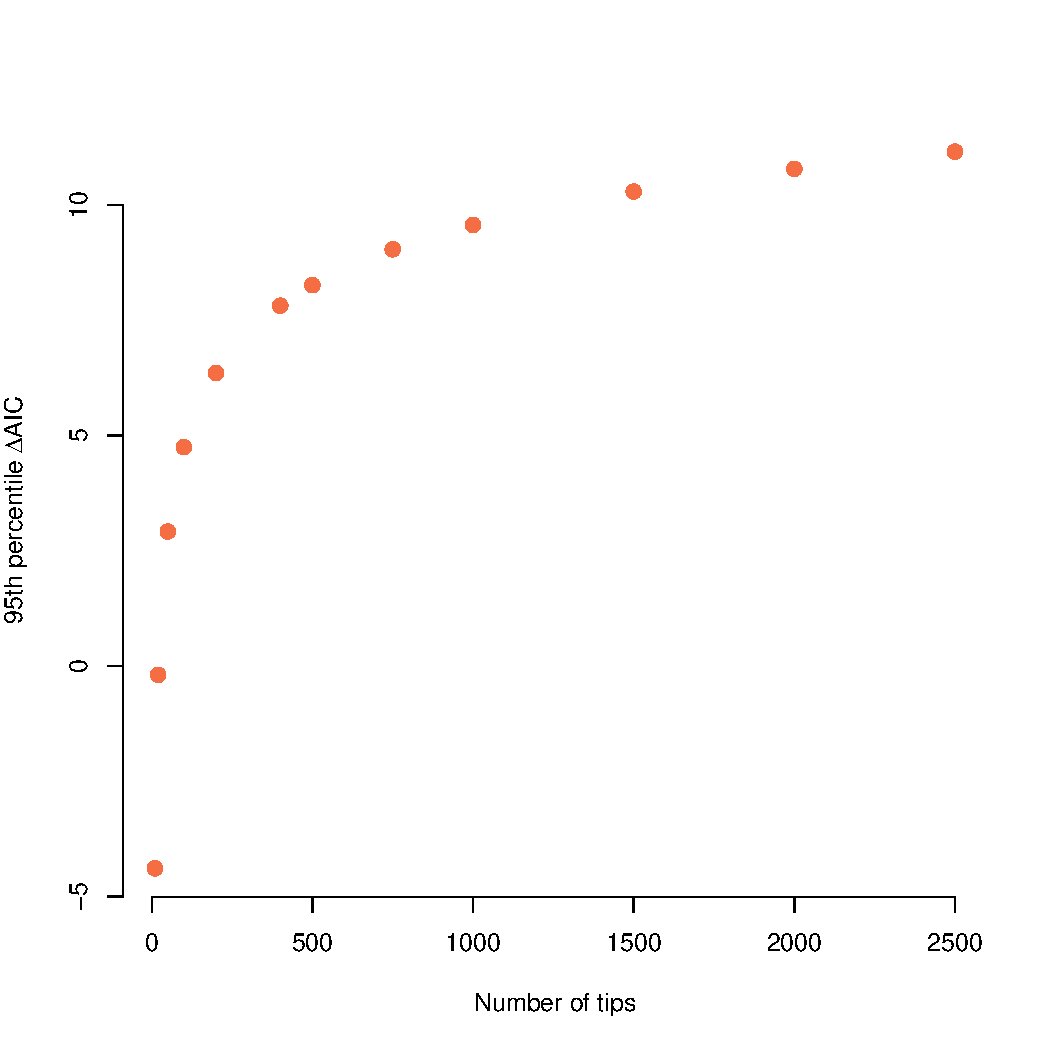
\includegraphics[width=\textwidth]{figs/BD_percentiles}
  \caption[Setting the \textsc{medusa} threshold via simulation]{The 95$^{th}$ percentile values for the difference in AICc scores ($\Delta$AICc) between the (incorrect) 1--shift model and the (true) 0-shift model plotted against simulated tree size. We fit a $x$-shifted power function to these points to estimate a AICc$_{t}$ with a Type-1 error rate of 0.05 for a given tree with $N$ tips.}
  \label{fig:medusa-threshold}
\end{figure}


\section{Concluding remarks}

In this note we provide a broad overview of the methods now available in \textsc{geiger}. We have not discussed some methods implemented in \textsc{geiger} \citep[e.g., `Congruification' for time-scaling large trees;][]{Eastman2013} and many of the nuances of the methods described here have been left out. We refer readers to associated publications and the package documentation for more information.

It is an exciting time for macroevolutionary research. We now have access to data sets of unparalleled size and a wide variety of new statistical approaches with which to analyze them. We hope that the software presented here will help researchers address some fundamental and long-standing questions in macroevolution. 
